\documentclass[a4paper,12pt]{article} 

%%% Работа с русским языком
\usepackage{cmap}					% поиск в PDF
\usepackage{mathtext} 				% русские буквы в фомулах
\usepackage[T2A]{fontenc}			% кодировка
\usepackage[utf8]{inputenc}			% кодировка исходного текста
\usepackage[english,russian]{babel}	% локализация и переносы

%%% Дополнительная работа с математикой
\usepackage{amsmath,amsfonts,amssymb,amsthm,mathtools, gensymb} % AMS
\usepackage{icomma} % "Умная" запятая: $0,2$ --- число, $0, 2$ --- перечисление

%%Таблица
\usepackage[table,xcdraw]{xcolor}
\usepackage{caption}
\usepackage{subcaption}
\usepackage{floatrow}
\floatsetup[table]{capposition=top}
\floatsetup[wrapfigure]{capposition=bottom}


%% Номера формул
\mathtoolsset{showonlyrefs=true} % Показывать номера только у тех формул, на которые есть \eqref{} в тексте.

%% Шрифты
\usepackage{euscript}	 % Шрифт Евклид
\usepackage{mathrsfs} % Красивый матшрифт

%% Свои команды
\DeclareMathOperator{\sgn}{\mathop{sgn}}

%% Перенос знаков в формулах (по Львовскому)
\newcommand*{\hm}[1]{#1\nobreak\discretionary{}
{\hbox{$\mathsurround=0pt #1$}}{}}

%% Стиль страницы
\usepackage{fancyhdr}

%% Для рисунков
\usepackage{graphicx}
\usepackage[export]{adjustbox}
\usepackage{float}
\usepackage{ragged2e}
\usepackage{wrapfig}

%Отступы и поля 
\textwidth=20cm
\oddsidemargin=-2cm
\topmargin=-2cm
\textheight=25cm

\pagestyle{fancy}
\begin{document}
\begin{titlepage}
\begin{center}
%\vspace*{1cm}
\large{\small ФЕДЕРАЛЬНОЕ ГОСУДАРСТВЕННОЕ АВТОНОМНОЕ ОБРАЗОВАТЕЛЬНОЕ\\ УЧРЕЖДЕНИЕ ВЫСШЕГО ОБРАЗОВАНИЯ \\ МОСКОВСКИЙ ФИЗИКО-ТЕХНИЧЕСКИЙ ИНСТИТУТ\\ (НАЦИОНАЛЬНЫЙ ИССЛЕДОВАТЕЛЬСКИЙ УНИВЕРСИТЕТ)\\ ФАКУЛЬТЕТ АЭРОКОСМИЧЕСКИХ ТЕХНОЛОГИЙ}
\vfill
\line(1,0){430}\\[1mm]
\huge{Лабораторная 5}\\
\huge\textbf{Числа с плавающей точкой (C)}\\
\line(1,0){430}\\[1mm]
\vfill
\begin{flushright}
\normalsize{Рогозин Владимир}\\
\normalsize{\textbf{Группа Б03-106}}\\
\end{flushright}
\end{center}
\end{titlepage}
\fancyhead[L] {Лабораторная 5}

\textbf{Пункт 1: Хранение целых чисел в памяти}

С помощью побитовых сдвигов через флаг $CF$ выведем сначала представление в памяти целого и целого беззнакового чисел. Код и результат программы представлены ниже
\begin{figure}[H]\label{fig: bits i and ui}
    \centering
    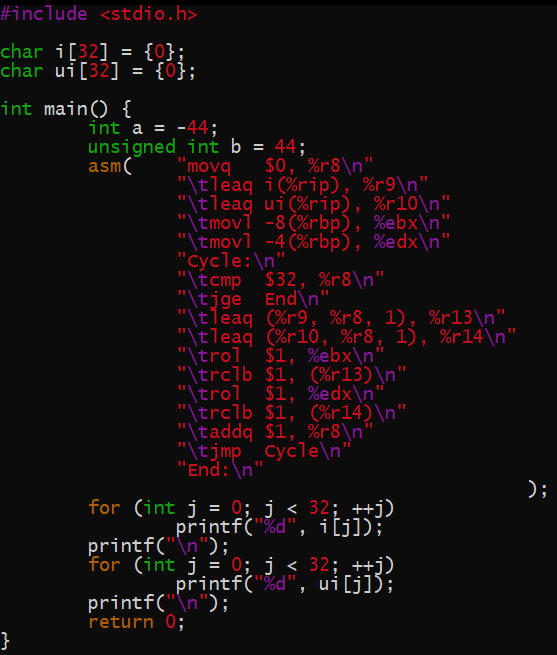
\includegraphics[width=0.7\textwidth]{Вставка побитового представления.png}
    \caption{Программа для вывода побитового представления}
\end{figure}
\begin{figure}[H]\label{fig: bits i and ui result}
    \centering
    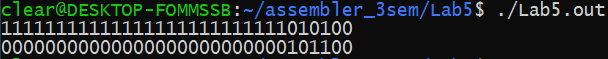
\includegraphics[width=0.7\textwidth]{Побитовое представление i ui.png}
    \caption{Результат работы программы}
\end{figure}
Видно, что положительные целые и числа типа \textit{unsigned int} хранятся в обычной двоичной записи, а отрицательные целые числа хранятся в виде дополнительного кода (инвертированная двоичная запись к которой прибавляется 1). 
\newpage

\textbf{Пункт 2: Хранение чисел c плавающей точкой и специальных символов}

Теперь попробуем таким способом вывести \textit{float}, \textit{double}, $\pm 0$ и $\pm\infty$. Сперва числа с плавающей точкой, воспользуемся программой из прошлого пункта, только вместо целых чисел будем подавать нецелые (для компьютера это все также набор единиц и нулей, так что главное начать сдвигать с нужной ячейки и нужное количество раз, то есть программа выведет корректное представление нецелых чисел в памяти).
\begin{figure}[H]\label{fig: bits d and f}
    \centering
    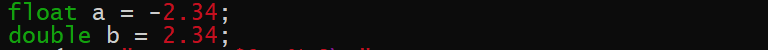
\includegraphics[width=0.7\textwidth]{Вставка f и d.png}
    \caption{\textit{float} и \textit{double} для вывода программе}
\end{figure}

\begin{figure}[H]\label{fig: bits d and f result}
    \centering
    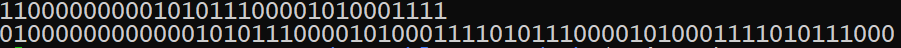
\includegraphics[width=0.7\textwidth]{Побитовое представление f d.png}
    \caption{\textit{float} и \textit{double} в памяти компьютера}
\end{figure}
Получили все так как и должно быть, первый бит отвечает за знак числа, затем 8 бит для \textit{float} и 11 бит для \textit{double}
хранят (порядок +127 или +1023) для \textit{float} и \textit{double}, и мантисса 23 бита и 52 бита соответственно.
Теперь то же самое только с бесконечностями.
\begin{figure}[H]\label{fig: bits pm inf}
    \centering
    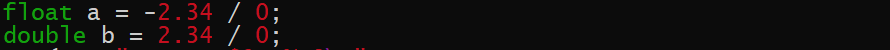
\includegraphics[width=0.7\textwidth]{Вставка pm inf.png}
    \caption{Создание $\pm \infty$ для вывода программе}
\end{figure}

\begin{figure}[H]\label{fig: bits pm inf result}
    \centering
    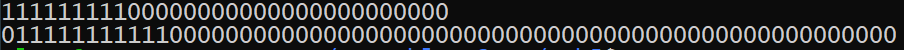
\includegraphics[width=0.7\textwidth]{Побитовое представление pm inf.png}
    \caption{$\pm \infty$ в памяти компьютера}
\end{figure}
Знак бесконечности определяется точно также как и у числа, то есть первым битом, мантисса нулевая, порядок максимально возможный, то есть все единички. То же самое сделаем для $\pm 0$.
\begin{figure}[H]\label{fig: bits pm 0}
    \centering
    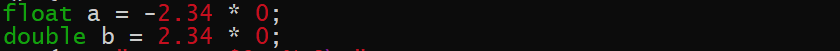
\includegraphics[width=0.7\textwidth]{Вставка pm 0.png}
    \caption{Создание $\pm 0$ для вывода программе}
\end{figure}

\begin{figure}[H]\label{fig: bits pm 0 result}
    \centering
    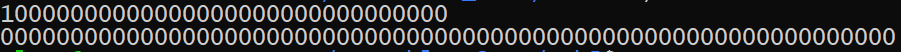
\includegraphics[width=0.7\textwidth]{Побитовое представление pm 0.png}
    \caption{$\pm 0$ в памяти компьютера}
\end{figure}
Первый бит все также указывает на знак нуля, мантисса состоит полностью из нулей, порядок тоже состоит только из нулей. Последним делом в этом пункте рассмотрим специальный символ NaN. Посмотрим как он хранится в памяти.  
\newpage

\begin{figure}[H]\label{fig: bits NaN}
    \centering
    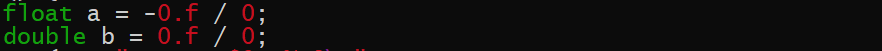
\includegraphics[width=0.7\textwidth]{Вставка NaN.png}
    \caption{Создание NaN для вывода программе}
\end{figure}

\begin{figure}[H]\label{fig: bits NaN result}
    \centering
    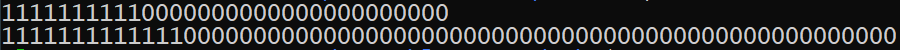
\includegraphics[width=0.7\textwidth]{Побитовое представление NaN.png}
    \caption{NaN в памяти компьютера}
\end{figure}
Видим, что NaN только один (первый разряд всегда единица), порядок как и в случае бесконечностей максимальный, то есть забор из единичек, но мантисса NaN отличается тем, что она ненулевая. В данном примере в мантиссе только на первом месте стоит 1, но вообще в ней может быть что угодно, отличное от нуля.

\textbf{Пункт 3: Переполнение мантиссы}

При сложении чисел с различными порядками сначала нужно привести их у одному порядку. Для этого мантисса числа с меньшим порядком сдвигается на нужное количество знаков вправо. Отсюда получаем, что при сложении чисел сильно разного порядка возможно переполнение мантиссы -- явление, при котором мантисса числа не влезает в отведённые ей 23 (52) бита.
\begin{figure}[H]\label{fig: Mantissa overflow code}
    \centering
    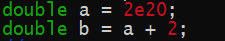
\includegraphics[width = 0.5\textwidth]{Переполнение мантиссы код.png}
    \caption{Складываем числа сильно разного порядка}
\end{figure}
\begin{figure}[H]\label{fig: Mantissa overflow result}
    \centering
    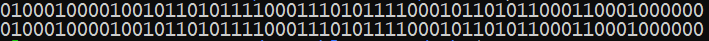
\includegraphics[width = 0.7\textwidth]{Переполнение мантиссы результат.png}
    \caption{Результат сложения; a сверху, b снизу}
\end{figure}
Видим, что $b$ стало равно $a$, а не $a + 2$. Мантисса вынуждена сдвинуться вправо слишком сильно, если различие больше чем на 52 двоичных порядка, то мантисса переполнится и станет нулевой, следовательно при сложении/вычитании один из операндов как бы становится нулём. 

\textbf{Пункт 4: Неассоциативность арифметических операций}

Теперь попробуем написать код, который продемонстрирует неассоциативность арифметических операций с $float$'ами. Очевидно нужно брать большие и маленькие числа. 
\begin{figure}[H]\label{fig: antiAssociation code}
    \centering
    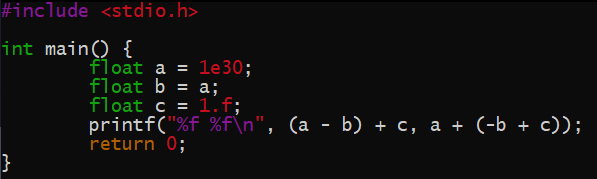
\includegraphics[width=0.7\textwidth]{Неассоциативность вставка.png}
    \caption{Код для демонстрации неассоциативности}
\end{figure}

\begin{figure}[H]\label{fig: antiAssociation result}
    \centering
    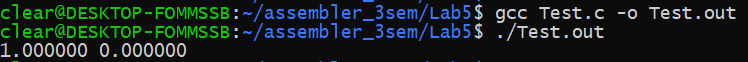
\includegraphics[width=0.7\textwidth]{Неассоциативность результат.png}
    \caption{Результат работы программы}
\end{figure}
Видим, что результаты действительно разные, хотя математика говорит, что должны быть одинаковыми. 

\textbf{Пункт 5: Числа с плавающей точкой в листинге}

Посмотрим на то, как производятся арифметические операции с $float$'ами и $double$'ами. Ниже представлены две программы и их ассемблерные листинги. Можем видеть, что команды те же что и для целых чисел, но с другими суффиксами. К тому же сами числа хранятся в специальных 128-битных регистрах \%xmm0, \%xmm1 и т.д. Всего таких регистров 8 штук. 

\begin{figure}[H]\label{fig: Code operations float and double}
    \subfloat[Арифм. операции $float$]{
    \begin{minipage}[t]{0.4\textwidth}
        \centering
        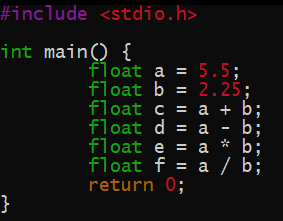
\includegraphics[width = 0.85\textwidth]{Операции float код.png}
    \end{minipage}}
    \subfloat[Арифм. операции $double$]{
    \begin{minipage}[t]{0.4\textwidth}
        \centering
        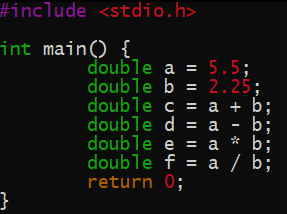
\includegraphics[width = 0.88\textwidth]{Операции double код.png}
    \end{minipage}}
\end{figure}

\begin{figure}[H]\label{fig: listing operations float and double}
    \subfloat[Листинг $float$]{
    \begin{minipage}[t]{0.4\textwidth}
        \centering
        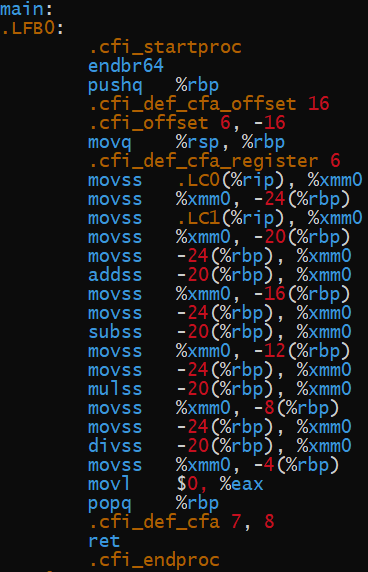
\includegraphics[width = 0.85\textwidth]{Операции float листинг.png}
    \end{minipage}}
    \subfloat[Листинг $double$]{
    \begin{minipage}[t]{0.4\textwidth}
        \centering
        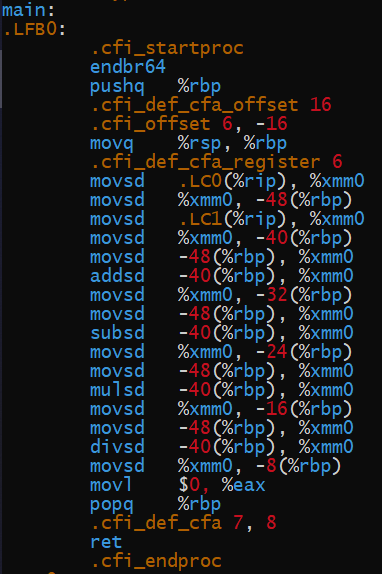
\includegraphics[width = 0.88\textwidth]{Операции double листинг.png}
    \end{minipage}}
\end{figure}

\textbf{Пункт 6: Вычисление числа $\pi$ различными формулами}

С помощью различных формул будем рассчитывать число $\pi$, запоминая значение на каждой итерации. По этим данным построим график числа $\pi$ от логарифма итераций. Для $float$'ов график получается такой же, на таком масштабе различия не видны.
\begin{figure}[H]\label{fig: Pi_double}
    \centering
    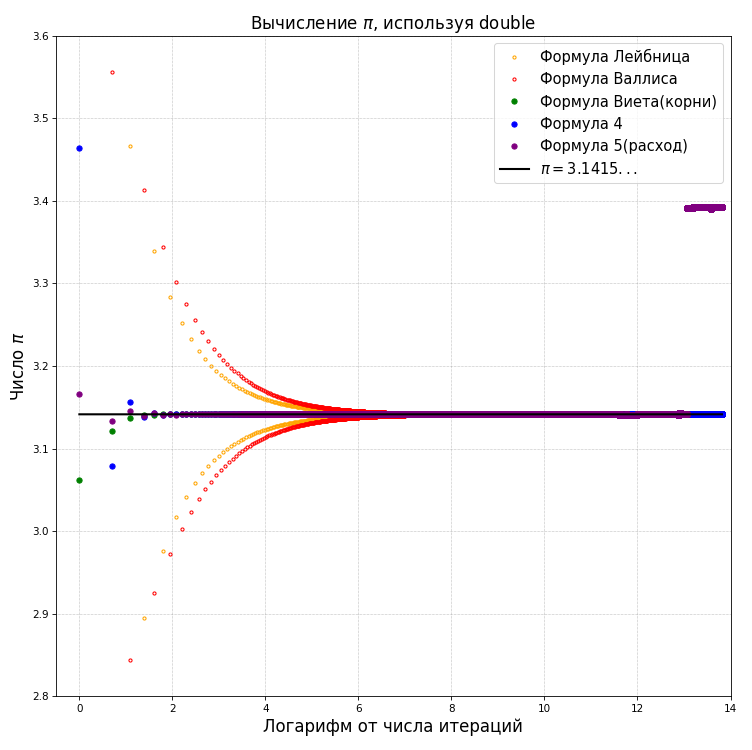
\includegraphics[width = \textwidth]{Pi_double.png}
\end{figure}
Из графика видно, что быстрее всего сходятся к $\pi$ формулы 3, 4. Формула 5 начинает расходиться в районе $e^{11,5}$ итерации, сильно начинает отличаться (уже в первом знаке после запятой) примерно на $e^{13}$ итерации.
\newpage 

\textbf{Пункт 7: Антипереполнение и денормализованные числа}

Теперь найдём минимальное по модулю значение для $float$ и $double$, для этого вычтем минимальное нормализованное число из следующего за ним, получим минимальное по модулю число. У минимального нормализованного числа должна быть нулевая мантисса и порядок 1 (с учётом вычета 127 или 1023). У минимального денормализованного числа должен быть нулевым порядок (с учётом вычета 127 или 1023) и минимальная ненулевая мантисса. В результате программы верхнее число -- минимальное нормализованное число, нижнее -- минимальное денормализованное. Для $float$ это $2^{-126}$ и $2^{-149}$ соответственно, для $double$ -- $2^{-1022}$ и $2^{-1074}$. Антипереполнение получим в следующем пункте, когда научимся отключать денормализованные числа.
\begin{figure}[H]\label{fig: minimum float code}
    \centering
    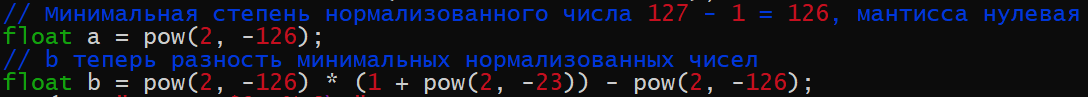
\includegraphics[width=0.7\textwidth]{Минимальный float вставка.png}
    \caption{Получаем минимальное значение $float$}
\end{figure}
\begin{figure}[H]\label{fig: minimum float result}
    \centering
    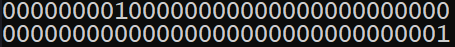
\includegraphics[width=0.7\textwidth]{Минимальный float результат.png}
    \caption{Минимальные значения $float$ в памяти}
\end{figure}

\begin{figure}[H]\label{fig: minimum double code}
    \centering
    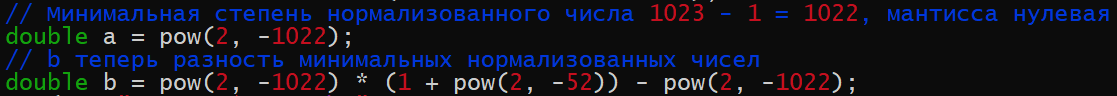
\includegraphics[width=0.7\textwidth]{Минимальный double вставка.png}
    \caption{Получаем минимальное значение $double$}
\end{figure}
\begin{figure}[H]\label{fig: minimum double result}
    \centering
    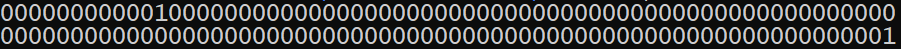
\includegraphics[width=0.7\textwidth]{Минимальный double результат.png}
    \caption{Минимальные значения $double$ в памяти}
\end{figure}

\textbf{Пункт 8: DAZ, FTZ и сравнение производительности}

DAZ и FTZ -- флаги которые влияют на появление/исчезновение денормализованных чисел. Включённый DAZ говорит обрабатывать денормализованные входные аргументы для операций, принимающих на вход числа с плавающей точкой, как 0, FTZ -- возвращать денормализованное значение как 0 для операций, где оно может появиться. Посмотрим на различия при наличии/отсутствии флагов.
\begin{figure}[H]\label{fig: FTZ code}
    \centering
    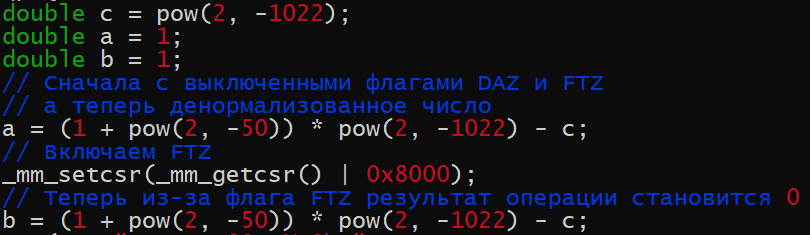
\includegraphics[width = 0.7\textwidth]{FTZ код.png}
    \caption{Программа с включённым FTZ}
\end{figure}
\begin{figure}[H]\label{fig: FTZ result}
    \centering
    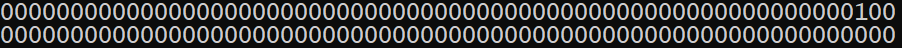
\includegraphics[width = 0.7\textwidth]{FTZ результат работы.png}
    \caption{Переменные a сверху и b снизу}
\end{figure}
Как и ожидалось, в результате операции вычитания получается денормализованное число, которое, если включён флаг FTZ, обнуляется. В ином случае оно остаётся ненулевым. 

\begin{figure}[H]\label{fig: DAZ code}
    \centering
    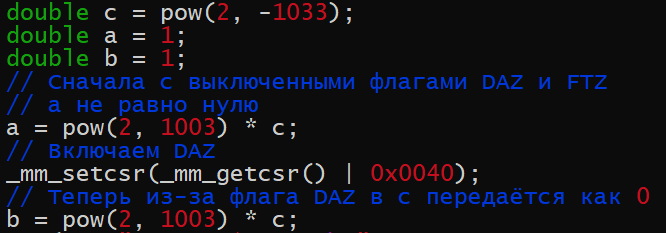
\includegraphics[width = 0.7\textwidth]{DAZ код.png}
    \caption{Программа с включённым DAZ}
\end{figure}
\begin{figure}[H]\label{fig: DAZ result}
    \centering
    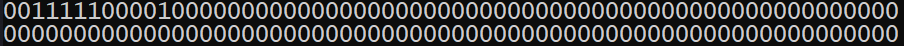
\includegraphics[width = 0.7\textwidth]{DAZ результат работы.png}
    \caption{Переменные a сверху и b снизу}
\end{figure}
Здесь, при взведённом флаге DAZ, в операцию умножения денормализованное число передаётся как 0, в результате умножения получается 0. В ином случае, как и должно быть в обычном режиме, получаем число, отличное от нуля. 

Далее, выясним влияет ли отключение денормализованных чисел на скорость операций с ними. Проверим для сложения $addss$ и умножения $divss$. Будем делать 20 итераций по 200 000 операций для каждого режима. Результаты представлены на картинках ниже.
\begin{figure}[H]\label{fig: Operations speed sum}
    \centering
    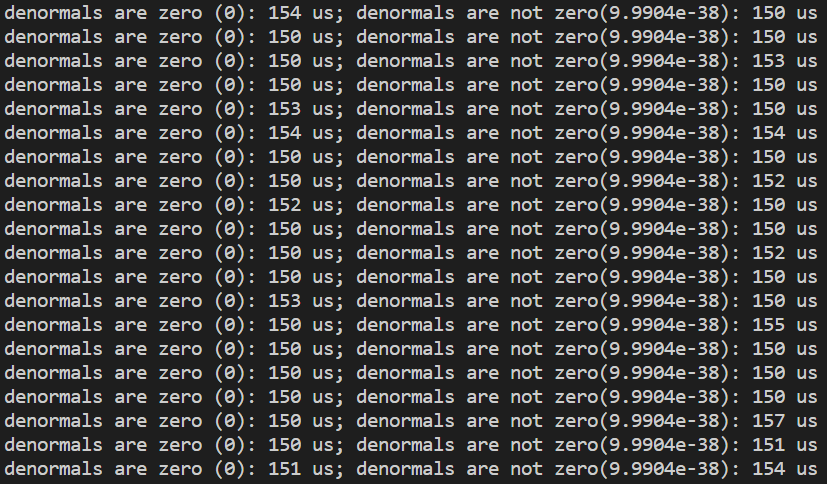
\includegraphics[width = 0.8\textwidth]{Сложение сравнение времени.png}
    \caption{Операция сложения $addss$}
\end{figure}
\begin{figure}[H]\label{fig: Operations speed div}
    \centering
    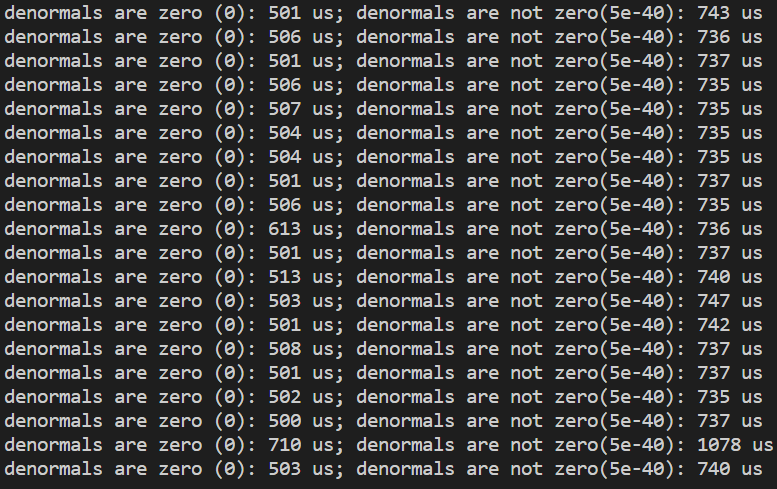
\includegraphics[width = 0.8\textwidth]{Деление сравнение времени.png}
    \caption{Операция деления $divss$}
\end{figure}
Как можем заметить, отключение денормализованных чисел ускоряет операцию деления, и никак не влияет на сложение чисел с плавающей точкой. Для операций вычитания и умножения ситуация аналогична сложению и делению соответственно.

\end{document}
